\documentclass[12pt]{beamer}
\usepackage[utf8]{inputenc}
\usepackage[dutch]{babel}
\usepackage{listings}
\usepackage{tabu}
\usepackage{booktabs}

\beamertemplatenavigationsymbolsempty
\AtBeginSection[]
{
    \begin{frame}
    \frametitle{Inhoudstafel}
    \tableofcontents[currentsection]
    \end{frame}
}

\newcommand{\gray}{\textcolor{gray}}
\newcommand{\bigoh}[1]{\mathcal{O}\left(#1\right)}
\newcommand{\constant}{\bigoh{1}}
\newcommand{\linear}{\bigoh{n}}

\definecolor{mygreen}{rgb}{0,0.6,0}
\definecolor{mygray}{rgb}{0.5,0.5,0.5}
\definecolor{mymauve}{rgb}{0.58,0,0.82}

\lstset{ %
  backgroundcolor=\color{white},   % choose the background color; you must add \usepackage{color} or \usepackage{xcolor}
  basicstyle=\tiny,        % the size of the fonts that are used for the code
  breakatwhitespace=false,         % sets if automatic breaks should only happen at whitespace
  breaklines=true,                 % sets automatic line breaking
  commentstyle=\color{mygreen},    % comment style
  deletekeywords={...},            % if you want to delete keywords from the given language
  escapeinside={\%*}{*)},          % if you want to add LaTeX within your code
  extendedchars=true,              % lets you use non-ASCII characters; for 8-bits encodings only, does not work with UTF-8
  frame=single,                    % adds a frame around the code
  keepspaces=true,                 % keeps spaces in text, useful for keeping indentation of code (possibly needs columns=flexible)
  keywordstyle=\color{blue},       % keyword style
  language=C++,                 % the language of the code
  morekeywords={*,...},            % if you want to add more keywords to the set
  numbers=left,                    % where to put the line-numbers; possible values are (none, left, right)
  numbersep=5pt,                   % how far the line-numbers are from the code
  numberstyle=\tiny\color{mygray}, % the style that is used for the line-numbers
  rulecolor=\color{black},         % if not set, the frame-color may be changed on line-breaks within not-black text (e.g. comments (green here))
  showspaces=false,                % show spaces everywhere adding particular underscores; it overrides 'showstringspaces'
  showstringspaces=false,          % underline spaces within strings only
  showtabs=false,                  % show tabs within strings adding particular underscores
  stepnumber=1,                    % the step between two line-numbers. If it's 1, each line will be numbered
  stringstyle=\color{mymauve},     % string literal style
  tabsize=2                      % sets default tabsize to 2 spaces
}

\title{Lineaire data structuren}
\subtitle{Tabellen, vectors en gelinkte lijsten}
\author{beOI Training}
\institute{
\includegraphics[height=12em]{../share/beoi-logo}}

\begin{document}

\frame{\titlepage}

\section{Tabellen en varianten}

\begin{frame}[fragile]
\frametitle{Tabel}
\begin{lstlisting}
#define MAX_N 10000
int tab[MAX_N];

int main() {
    tab[1234] = 100;
    tab[1234]; // 100
    tab[5678]; // 0
}
\end{lstlisting}
\begin{itemize}
\item Grootte van de tabel vooraf bepaald bij de compilatie
\item Toegang tot een willekeurig element: $\constant$
\item \textit{Buiten functies} worden elementen op 0 geïnitialiseerd
\end{itemize}
\end{frame}

\begin{frame}[fragile]
\frametitle{Bitset}
C++ : \texttt{bitset} \\
Java : \texttt{BitSet}
\begin{lstlisting}
bitset<MAX_N> tab; // bool tab[MAX_N];
tab[1234] = true;

bitset<4> b1(string("1100")),
          b2(string("0101"));
b1 | b2; // 1101
b1 & b2; // 0100
b1 >> 1; // 0110
\end{lstlisting}
\begin{itemize}
\item Zoals een tabel van booleans
\item 8 keer compacter
\item Bit operaties tot 64 keer sneller
\item Zie internet voor een volledige lijst van operaties
\end{itemize}
\end{frame}

\begin{frame}[fragile]
\frametitle{Dynamische tabel: werking}
{\setlength{\parskip}{.9em}
Als er onvoldoende plaats is, wordt de lengte verdubbeld

\def\arraystretch{1.3}

\begin{tabu} to .175\textwidth {|X[c]|X[c]|}
\hline
1 & \\
\hline
\end{tabu}
\hfill Capaciteit = 2

\begin{tabu} to .175\textwidth {|X[c]|X[c]|}
\hline
1 & 2 \\
\hline
\end{tabu}

\begin{tabu} to .35\textwidth {|X[c]|X[c]|X[c]|X[c]|}
\hline
1 & 2 & 3 & \\
\hline
\end{tabu}
\hfill Capaciteit = 4

\begin{tabu} to .35\textwidth {|X[c]|X[c]|X[c]|X[c]|}
\hline
1 & 2 & 3 & 4 \\
\hline
\end{tabu}

\begin{tabu} to .7\textwidth {|X[c]|X[c]|X[c]|X[c]|X[c]|X[c]|X[c]|X[c]|}
\hline
1 & 2 & 3 & 4 & 5 & & & \\
\hline
\end{tabu}
\hfill Capaciteit = 8} %\setlength
\end{frame}

\begin{frame}[fragile]
\frametitle{Dynamische tabel: in de praktijk}
C++ : \texttt{vector} \\
Java : \texttt{ArrayList<E>}
\begin{lstlisting}
vector<int> vec(8, -1); // initialize to -1
vec[5] += vec[2];       // -2
vec.push_back(5);
vec.push_back(19);
vec.pop_back();
vec.back();             // 5
\end{lstlisting}
\begin{itemize}
\item Omvang kan toenemen en afnemen
\item Toegang tot een willekeurig element: $\constant$
\item Toevoegen/verwijderen van een element \textbf{op het einde}: $\constant$
\item Ergens anders toevoegen/verwijderen: $\linear$
\end{itemize}
\end{frame}

\section{Gelinkte lijsten}

\begin{frame}[fragile]
\frametitle{Gelinkte lijst: concept}
Knopen worden gelinkt met wijzers (pointers)
\begin{figure}
\centering
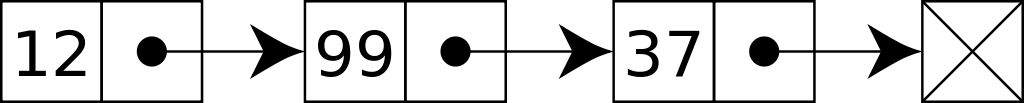
\includegraphics[width=.8\textwidth]{img/singly-linked}
\end{figure}
\begin{itemize}
\item Elke knoop weet waar de volgende is
\end{itemize}
\begin{lstlisting}
struct Node {
    int value;
    Node *next; // link (pointer)
};
\end{lstlisting}
\end{frame}

\begin{frame}[fragile]
\frametitle{Gelinkte lijst: doorlopen}
Beginnen bij de eerste knoop en de wijzers volgen
\begin{figure}
\centering
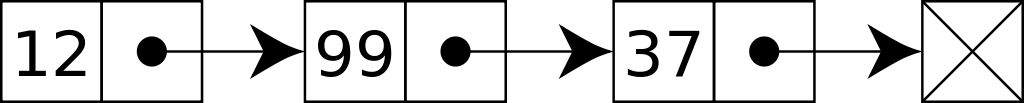
\includegraphics[width=.6\textwidth]{img/singly-linked}
\end{figure}
In de laatste knoop heeft de wijzer de waarde NULL:
\begin{lstlisting}
Node *cur = start;   // always keep the first node!
while (cur != NULL) {
    cur->value;      // access value
    cur = cur->next; // switch pointer to next
}
\end{lstlisting}
\end{frame}

\begin{frame}[fragile]
\frametitle{Gelinkte lijst: toevoegen}
Je moet maar twee wijzers veranderen
\begin{figure}
\centering
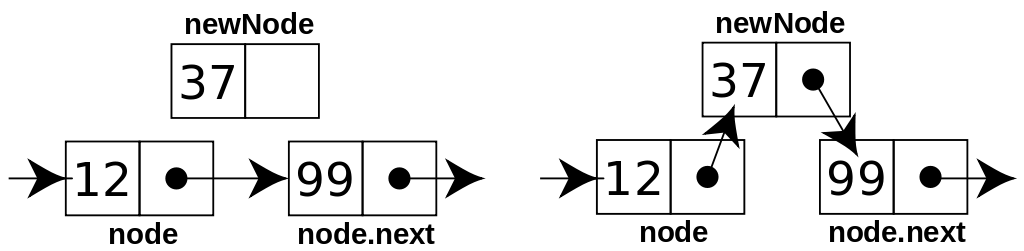
\includegraphics[width=.9\textwidth]{img/insert-node}
\end{figure}
\begin{lstlisting}
void insertAfter(Node *node, Node *new_node) {
    new_node->next = node->next;
    node->next = new_node;
}
\end{lstlisting}
\end{frame}

\begin{frame}[fragile]
\frametitle{Gelinkte lijst: verwijderen}
Verander de wijzer en geef geheugen vrij van de verwijderde knoop
\begin{figure}
\centering
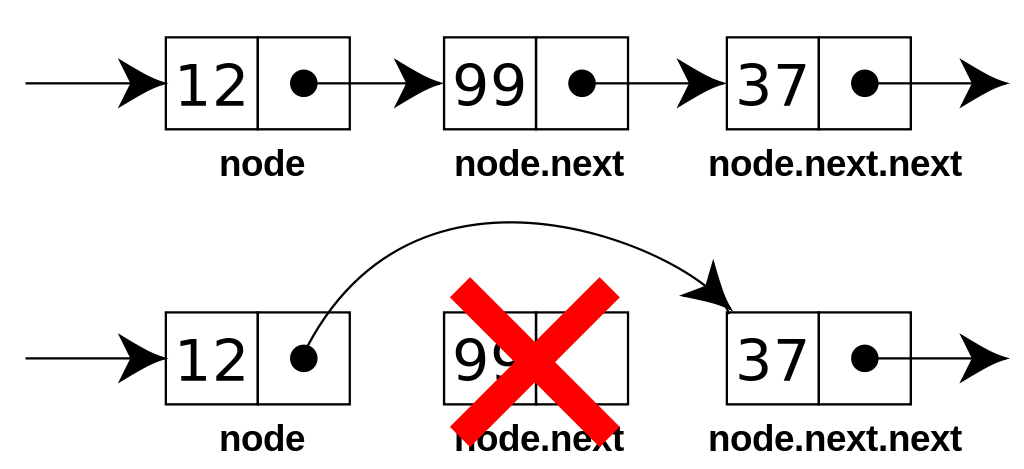
\includegraphics[width=.6\textwidth]{img/remove-node}
\end{figure}
\begin{lstlisting}
void removeAfter(Node *node) {
    Node *toRemove = node->next;
    node->next = node->next-next; // bypass
    free(toRemove);
}
\end{lstlisting}
\end{frame}

\begin{frame}[fragile]
\frametitle{Gelinkte lijst: beperkingen}
\begin{figure}
\centering
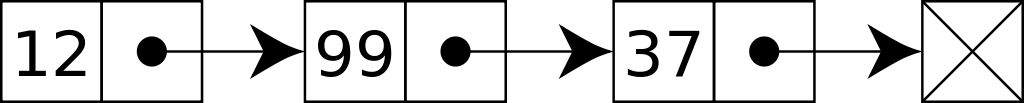
\includegraphics[width=.8\textwidth]{img/singly-linked}
\end{figure}
Met een enkel gelinkte lijst:
\begin{itemize}
\item Toevoegen/verwijderen in het begin van de lijst: $\constant$
\item Toevoegen/verwijderen op een \textbf{gegeven} positie : $\constant$
\end{itemize}
Als we ook het einde onthouden:
\begin{itemize}
\item Toevoegen op het einde: $\constant$
\item Verwijderen op het einde : $\linear$
\end{itemize}
\end{frame}

\begin{frame}[fragile]
\frametitle{Dubbel gelinkte lijsten}
Wijzers in de twee richtingen!
\begin{figure}
\centering
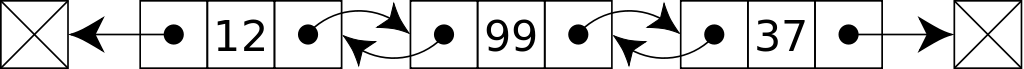
\includegraphics[width=.8\textwidth]{img/doubly-linked}
\end{figure}
\begin{itemize}
\item Doorlopen in de twee richtingen
\item Verwijderen op het einde van de lijst in $\constant$
\item Iets meer geheugengebruik
\end{itemize}
\begin{lstlisting}
struct Node
{
    int value;
    Node *prev, *next; // two pointers
};
\end{lstlisting}
\end{frame}

\begin{frame}[fragile]
\frametitle{Gelinkte lijst: in de praktijk}
C++ : \texttt{list} \\
Java : \texttt{LinkedList<E>}
\begin{lstlisting}
list<int> l;
list<int>::iterator it;

l.push_back(3);  // 3
it = l.begin();  // ^ points to 3
l.push_back(4);  // 3 4
l.push_front(1); // 1 3 4
l.insert(it, 2); // 1 2 3 4 (inserts before 3)
l.pop_front();   // 2 3 4
l.pop_back();    // 2 3
\end{lstlisting}
\begin{itemize}
\item De data structuur \texttt{list<>} is een dubbel gelinkte lijst
\item Posities onthouden met \texttt{iterators}
\item Allemaal in $\constant$
\end{itemize}
\end{frame}

\section{De rij en de stapel}

\begin{frame}
\frametitle{Rij: concept}
\begin{itemize}
\item Zoals een rij in een winkel
\item We voegen aan het einde dingen toe en halen bij het begin dingen weg
\item First In First Out
\end{itemize}
\begin{figure}
\centering
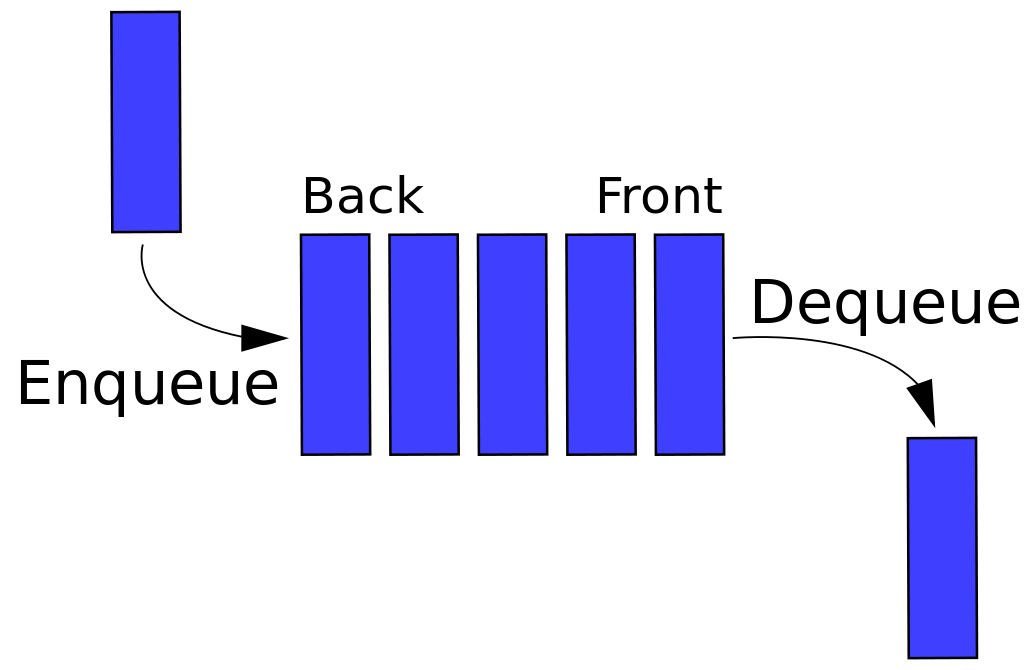
\includegraphics[width=.6\textwidth]{img/queue}
\end{figure}
\end{frame}

\begin{frame}[fragile]
\frametitle{Rij: in de praktijk}
C++ : \texttt{queue} \\
Java : \texttt{Queue<E>}
\begin{itemize}
\item Toevoegen aan het einde, weghalen bij het begin $\Rightarrow$ gelinkte lijst
\item Allemaal in $\constant$
\end{itemize}
\begin{lstlisting}
queue<int> q;
q.push(1);
q.push(2);
q.front(); // 1
q.pop();
q.front(); // 2
\end{lstlisting}
\end{frame}

\begin{frame}
\frametitle{Stapel: concept}
\begin{itemize}
\item Zoals een stapel pannekoeken
\item We voegen bovenaan toe en halen bovenaan weg
\item Laatst gebakken wordt eerst opgegeten (Last In First Out)
\end{itemize}
\begin{figure}
\centering
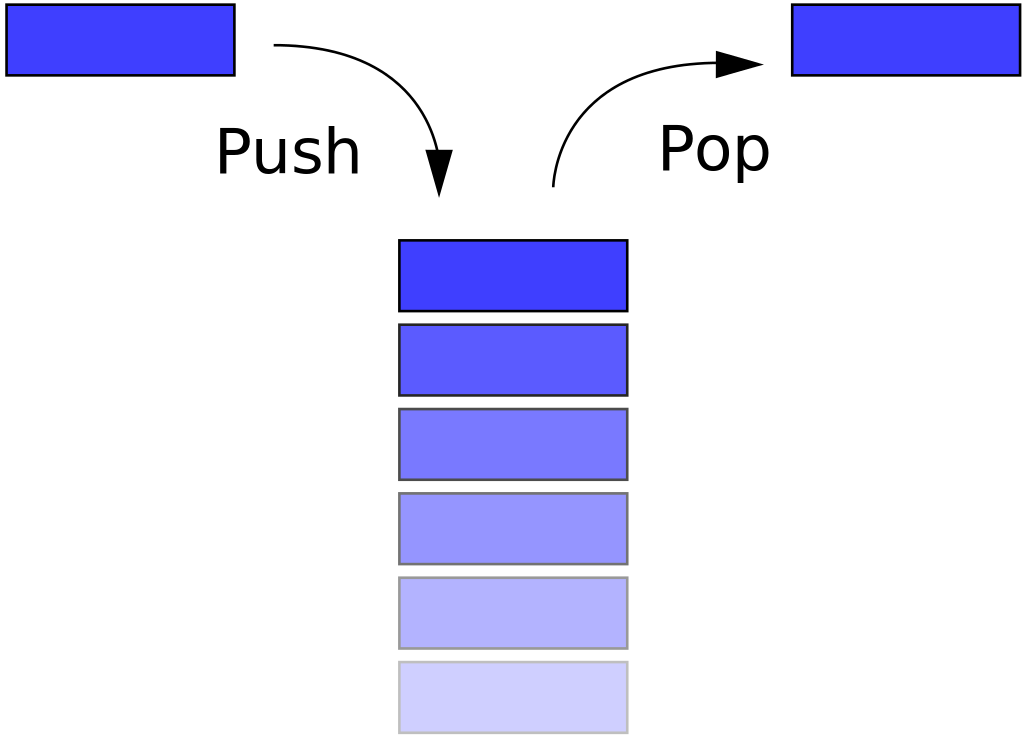
\includegraphics[width=.5\textwidth]{img/stack}
\end{figure}
\end{frame}

\begin{frame}[fragile]
\frametitle{Stapel: in de praktijk}
C++ : \texttt{stack} \\
Java : \texttt{Stack<E>}
\begin{itemize}
\item Toevoegen en verwijderen op het einde $\Rightarrow$ gelinkte lijst \emph{of vector}
\item Allemaal in $\constant$
\end{itemize}
\begin{lstlisting}
stack<int> q;
q.push(1);
q.push(2);
q.top(); // 2
q.pop();
q.top(); // 1
\end{lstlisting}
\end{frame}

\section{De goede data structuur kiezen}

\begin{frame}
\frametitle{Keuze: speciale data structuren}
Data structuren voor specifieke noden:
\begin{itemize}
\item Aan de ene kant toevoegen en aan de andere kant weghalen $\Rightarrow$ \textbf{rij}
\item Toevoegen en weghalen aan dezelfde kant $\Rightarrow$ \textbf{stapel}
\item Booleans, speciale operaties (en, of, shift...)  $\Rightarrow$ \textbf{bitset}
\end{itemize}

~

In het andere geval, zie volgende slide!
\end{frame}

\begin{frame}
\frametitle{Keuze: tabellen, vectors en gelinkte lijsten}
``Toevoegen'' = toevoegen of verwijderen
\begin{center}
\begin{tabu}{l|cccc}
\toprule
Data structuur & Indexatie & Toevoegen einde & Toevoegen midden \\
\midrule
Tabel & $\constant$ & $\linear$ & $\linear$ \\
Vector& $\constant$ & $\constant$ & $\linear$ \\
Gelinkte lijst & $\linear$ & $\constant$ & $\constant$ \\
\bottomrule
\end{tabu}
\end{center}
\begin{itemize}
\item Toevoegen in het midden nodig (zeldzaam) $\Rightarrow$ \textbf{gelinkte lijst}
\item Maximale grootte onbekend $\Rightarrow$ \textbf{vector}
\item Alle andere gevallen $\Rightarrow$ \textbf{tabel} (sneller)
\end{itemize}
\end{frame}

\begin{frame}
\frametitle{Bronnen van de figuren}
\begin{itemize}
\item \url{https://commons.wikimedia.org/wiki/File:Singly-linked-list.svg}
\item \url{https://commons.wikimedia.org/wiki/File:CPT-LinkedLists-addingnode.svg}
\item \url{https://en.wikipedia.org/wiki/File:CPT-LinkedLists-deletingnode.svg}
\item \url{https://en.wikipedia.org/wiki/File:Doubly-linked-list.svg}
\item \url{https://en.wikipedia.org/wiki/File:Data_Queue.svg}
\item \url{https://en.wikipedia.org/wiki/File:Data_stack.svg}
\end{itemize}
\end{frame}

\end{document}
